\documentclass{article}
\usepackage{graphicx}
\usepackage{wrapfig}

\begin{document}
\title{Factors Affecting Extinction}

\begin{figure}
    
\includegraphics[width=\linewidth]{ITU.jpg}
\end{figure}
\maketitle
\author{Rinalds Lipenitis \and Jakub Mráz \and
Adam Rosenørn \and Costel Gutu \and Richard Kentoš}
\begin{center}
\date{March 2023}
\end{center}

\newpage

\section{Abstract}

This study investigates the factors affecting extinction times of bird species on 16 islands around Britain. We analyze a dataset containing measurements on breeding pairs of land-bird species, including the average time of extinction, the average number of nesting pairs, size (large or small), and migratory status (migrant or resident). The primary goal is to determine the impact of these factors on extinction times, while accounting for the number of nesting pairs. Using linear regression models, we identify significant relationships between extinction times and the predictor variables. The study highlights outliers with unusually large extinction times compared to other species.

\section{Introduction}

The risk of extinction among bird species has become an increasing concern for conservationists and ecologists. Understanding the factors that influence extinction times can help guide conservation efforts and prioritize resources. In this study, we analyze a dataset collected from 16 islands around Britain over several decades, focusing on breeding pairs of land-bird species. The dataset includes measurements on the average time of extinction, the average number of nesting pairs, bird size (large or small), and migratory status (migrant or resident).

Previous research suggests that species with a large number of nesting pairs tend to remain longer before becoming extinct. In this study, we aim to investigate whether bird size and migratory status also play a role in extinction times, after accounting for the number of nesting pairs. Additionally, we identify species with unusually small or large extinction times compared to other species with similar values for the explanatory variables. This information can help conservationists understand the underlying factors contributing to bird extinction and develop targeted strategies to protect vulnerable species.

\section{Fitting the Full Model (ex. 1)}
To begin with, we fitted the full model with all interactions between the variables present, allowing us to investigate the possible effects of these interactions,
and deciding whether they are statistically significant or not. This model assigns the value 1 to the Resident and Small categorites and 0 to their counterparts.

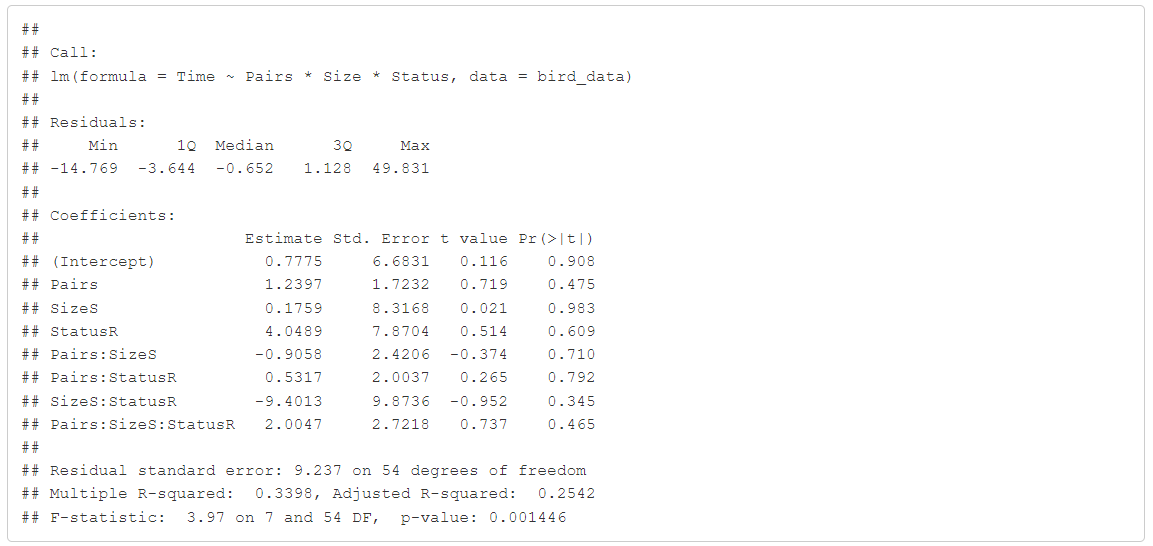
\includegraphics[scale=0.5]{tables/all-multiplied.png}


\begin{center}
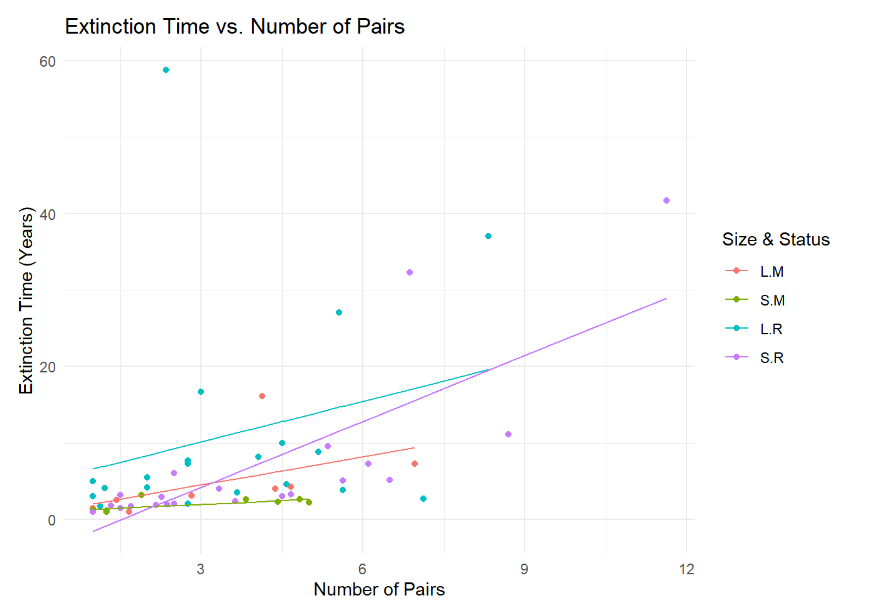
\includegraphics[scale=0.5]{graphs/graph1.png}
\end{center}

\section{Examining the Residuals (ex. 2)}

We examined the dataset for possible transformations and outliers by creating a residual plot from the fit of the full model. Based on this plot, we identified potential issues and assessed the need for data transformations.

\begin{center}
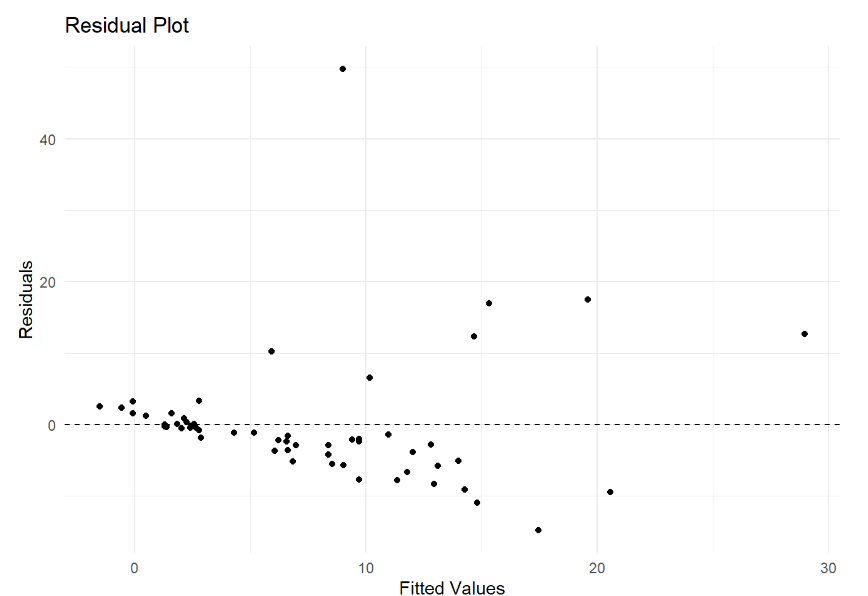
\includegraphics[scale=0.5]{graphs/residual.png}
\end{center}


When examining the residuals, we looked for: \\

Homoscedasticity: The variance of the residuals becomes bigger and bigger as the value
being fitted (number of pairs + extinction time) goes up.

Independence: There appears to be a slight downward slope pattern. \\

Biggest Outlier: \\
Species: Raven \\
Time: 58.82 \\
Pairs: 2.35 \\
Size: L \\
Status: R \\

Normality:

\begin{center}
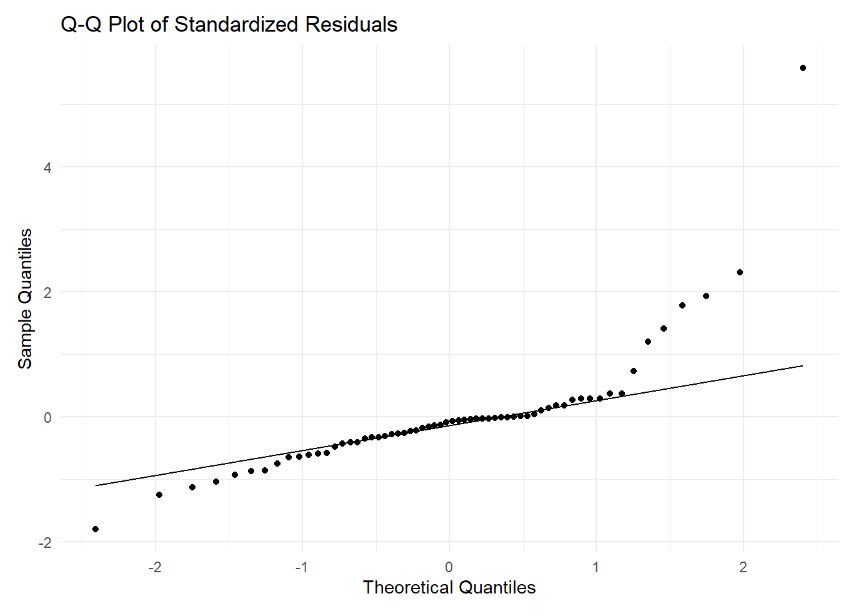
\includegraphics[scale=0.5]{graphs/qq-residuals.png}
\end{center}

The residuals appear to be normally distributed except for the lower and upper ends, where they become more skewed, this suggests that a data transformation may be necessarry.


\section{Data Transformation (ex. 3)}

Since it was apparent that some data transformation was necessary, we explored different methods of transforming the time variable, namely logarithmic, quadratic, and reciprocal.

\begin{center}
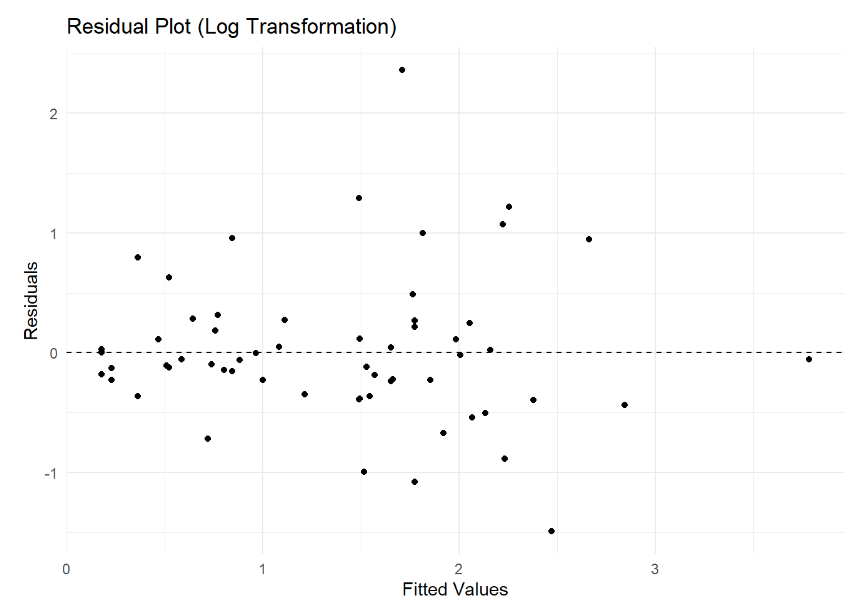
\includegraphics[scale=0.5]{graphs/graph-log.png}
\end{center}

\begin{center}
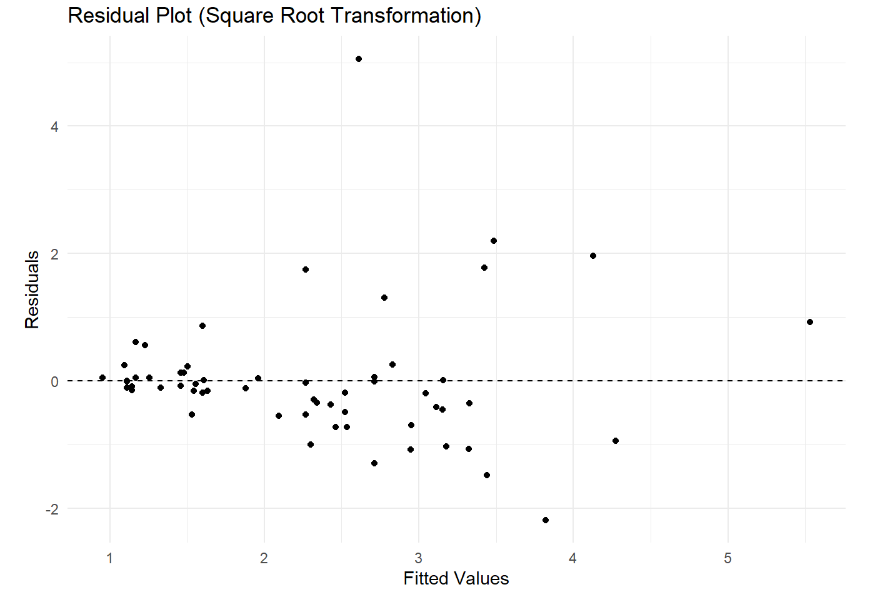
\includegraphics[scale=0.5]{graphs/graph-sqrt.png}
\end{center}

\begin{center}
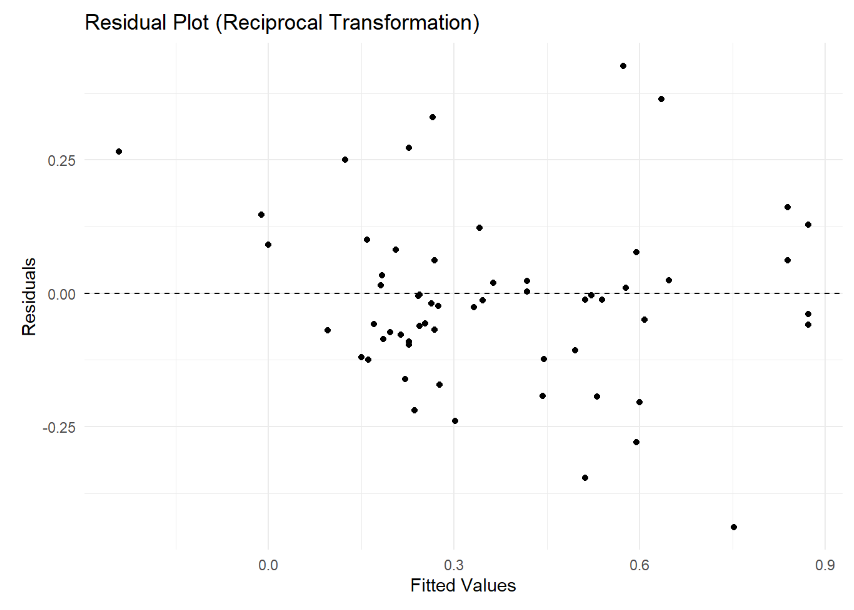
\includegraphics[scale=0.5]{graphs/graph-over.png}
\end{center}

Immediately, we can tell that the square transformation does not improve the model. To compare the log and reciprocal transformation, we will use Q-Q plots again.

Based on the Q-Q plots, the log transformation seems to be the best fit for the majority of the fitted data points.

\section{Approach Towards Outliers (ex. 4)}
Since there were some large outliers, such as the Raven species, it was important for us to decide our approach towards them.

Results can be significantly impacted by the outlier in each end of the scale. Outliers can also affect the measures of the central tendency, more specifically mean, median and mode. Moreover, they can also affect standard deviation and range - the spread of the data.

We believe that is is vital for us to keep the outliers in the dataset for various reasons:

1. Outliers provide important information about the data distribution. To be more specific, they can indicate the presence of extreme or unusual values, which might be beneficial for understanding the range and variability of our data. For instance,  the outlier for the Peregrine species in this dataset indicates that it has a much lower average time until it becomes extinct than the other species. This could also be because of the specific environmental or ecological factors.

2. Preventing loss of information and biased analysis. Outliers may be representing rare but important occurrences that we should not leave out. Removing them might result in a distorted view of the true data distribution and lead to incorrect conclusions. For instance, if we decided to remove the outlier for the Raven species in this dataset, we would miss the fact that it has much longer average extinction time than the other species.

3. Allowing more robust statistical analysis. Methods such as robust regression or non-parametric tests are able to handle outliers and provide more accurate results.

We therefore think that is is inevitable to keep outliers in our dataset and carefully consider how they impact the results. Rather than removing them, it may be better to investigate why they exist in the first place and how they may affect the analysis.


\section{Exploring Further Data Transformations (ex. 5)}
We then explored the possibility of log-transforming the pairs variable. Transformation of a variable is often done to linearize a relationship between two variables which is not linear in its original form. However, in this question we are specifically asked to assess whether there are linear relationships between log('time') and 'pairs' in all possible combinations of 'size' and 'migratory status'.

\begin{center}
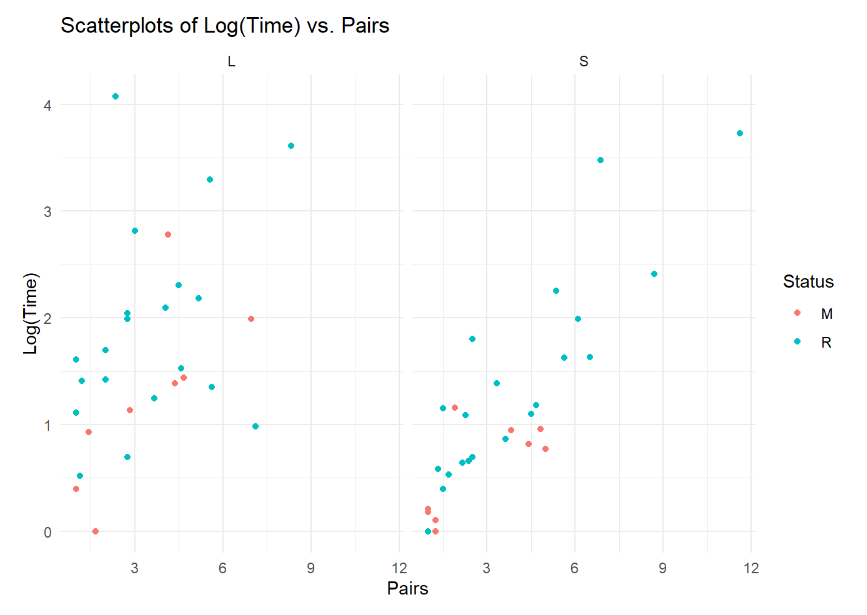
\includegraphics[scale=0.5]{graphs/graph5.png}
\end{center}

The relationship between log(Time) and Pairs does appear to be a positive linear relationship, thus indicating that a transformation of Pairs is not needed.

The relationship also appears to be more linear than with log-transformed Pairs, as shown below, where a slight curve pattern emerges.



\section{Exploring Variable Interactions (ex. 6)}

Next, we did an analysis as to whether the interactions present in our full model were statistically significant enough for us to preserve. This was done with the help of two methods.

\subsection*{6.1}
The first method was analysis the R-generated summary of our full model.
\begin{center}
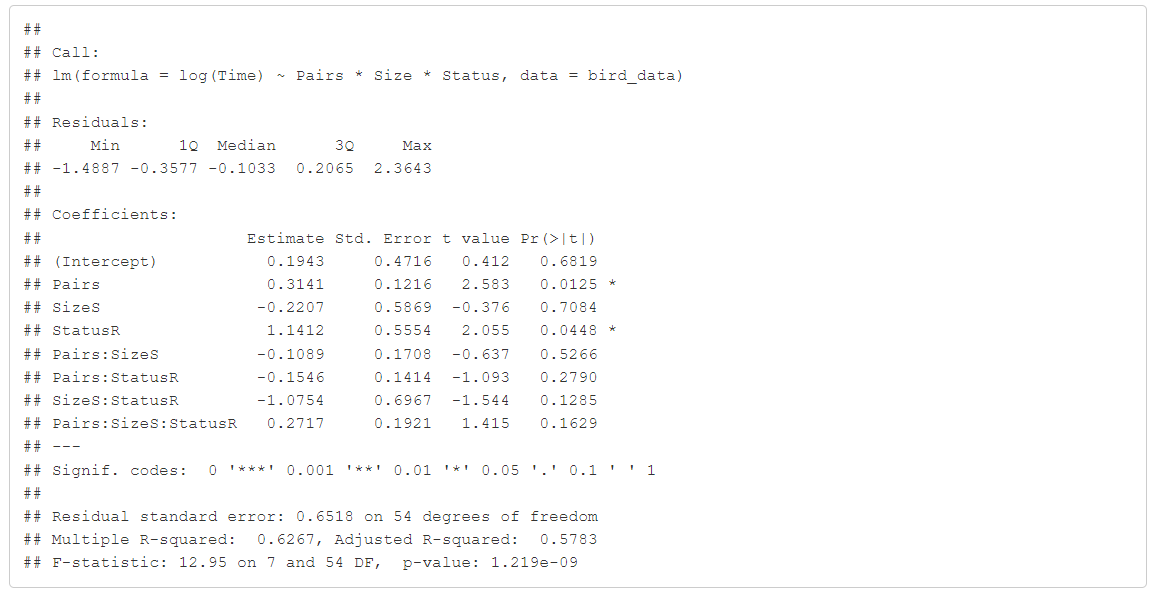
\includegraphics[scale=0.5]{tables/log-time.png}
\end{center}


To determine whether the slopes are equal for all combinations of “size” and “migratory status,” we examined the coefficients for the interaction terms Pairs:Size, Pairs:Status, and Pairs:Size:Status. If the interaction terms are not statistically significant (i.e., their p-values are larger than a chosen significance level, typically 0.05), it suggests that the slopes are not significantly different between the four combinations of “size” and “migratory status.” \\

Pairs:SizeS: The coefficient is -0.1089 with a p-value of 0.5266, which is not statistically significant at a 0.05 significance level. \\

Pairs:StatusR: The coefficient is -0.1546 with a p-value of 0.2790, which is not statistically significant at a 0.05 significance level. \\

Pairs:SizeS:StatusR: The coefficient is 0.2717 with a p-value of 0.1629, which is not statistically significant at a 0.05 significance level. \\

Since none of the interaction terms are statistically significant, there is not enough evidence to conclude that the slopes for all four combinations of “size” and “migratory status” are different. This suggests that the relationship between “Pairs” and log(“Time”) may not be significantly different among the four groups based on “size” and “migratory status”. However, it is essential to note that a lack of statistical significance does not necessarily mean the slopes are equal; it indicates that there isn’t enough evidence to reject the null hypothesis that the slopes are equal.

\subsection*{6.2}

The second method was using nested models and R's ANOVA analysis.

Nested models are a series of models where each model is a subset of the previous one. This approach helps in assessing the contribution of variables and their interactions to the overall model fit. To create nested models, start with the simplest model and gradually add variables and interaction terms to evaluate their contributions.


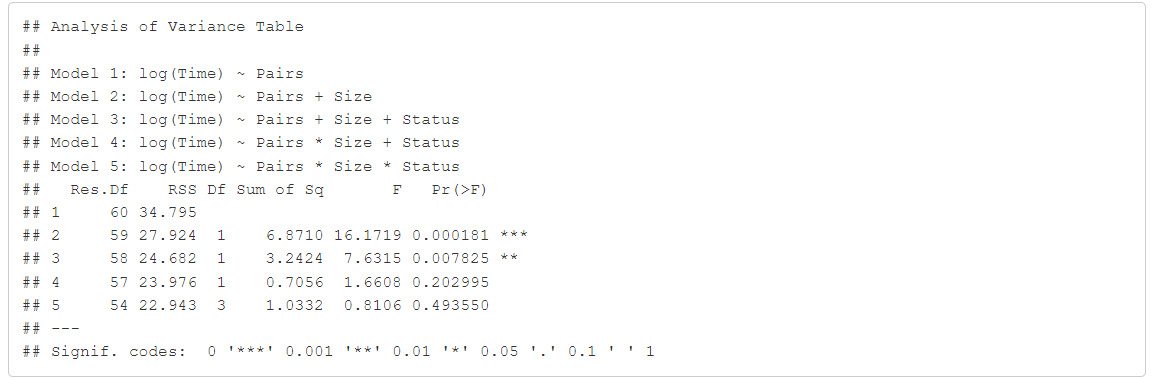
\includegraphics[scale=0.5]{tables/variance-table.png}


When we move from Model 1 to Model 2 (adding the Size variable), the p-value is 0.000181 (significant at the 0.05 level). This indicates that adding the Size variable significantly improves the model fit.

When we move from Model 2 to Model 3 (adding the Status variable), the p-value is 0.007825 (significant at the 0.05 level). This suggests that adding the Status variable significantly improves the model fit.

When we move from Model 3 to Model 4 (adding the Pairs * Size interaction term), the p-value is 0.202995 (not significant at the 0.05 level). This suggests that adding the Pairs * Size interaction term does not significantly improve the model fit.

When we move from Model 4 to Model 5 (adding the Pairs * Size * Status interaction term), the p-value is 0.493550 (not significant at the 0.05 level). This indicates that adding the Pairs * Size * Status interaction term does not significantly improve the model fit.

Based on the ANOVA results, it seems that Model 3 (Time ~ Pairs + Size + Status) is the most appropriate model for this dataset, as adding interaction terms does not significantly improve the model fit.

\section{Reducing the Model (ex. 7)}
Based on the findings from previous items, we can create a reduced model using just the Pairs, Size, and Status variables, without interaction terms.


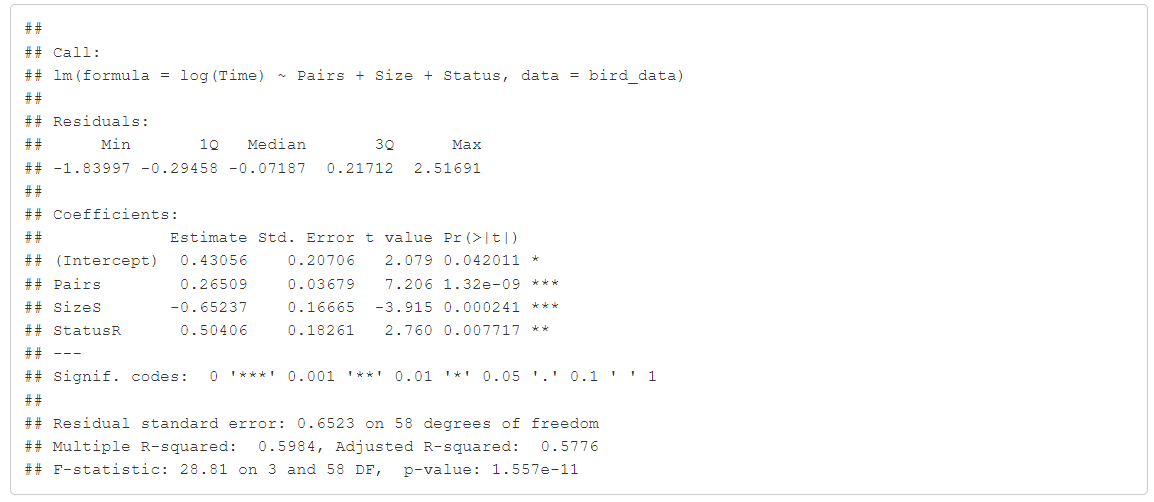
\includegraphics[scale=0.5]{tables/all-added.png}


\begin{center}
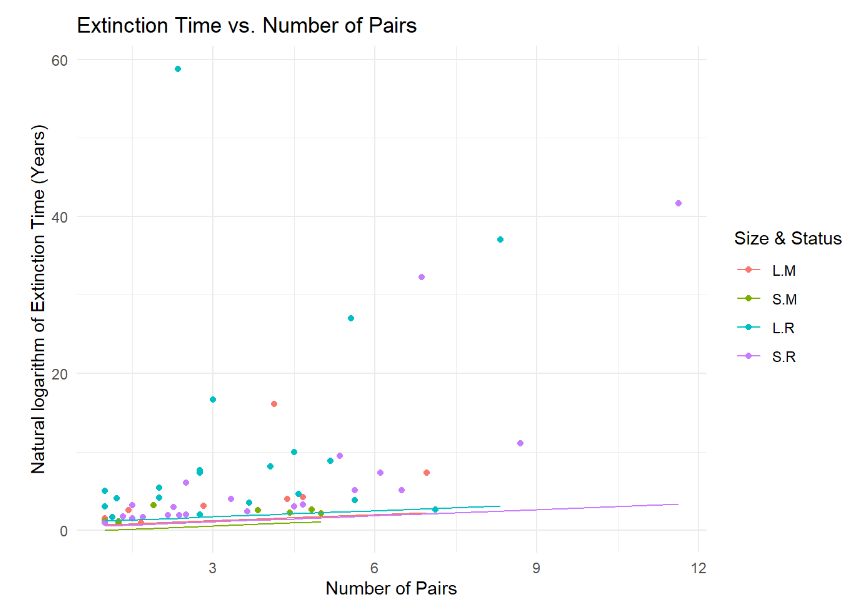
\includegraphics[scale=0.5]{graphs/graph7.png}
\end{center}

\section{Conclusion (ex. 8)}

After analyzing the data and accounting for the number of nesting pairs,
we can conclude that the number of nesting pairs has a significant
impact on the time it takes for a species to become extinct. Larger
numbers of nesting pairs tend to result in longer times before
extinction.

However, when considering the size and migratory status of species,
their individual effects on extinction time are less clear. We could not
establish a strong relationship between these factors and the time to
extinction, indicating that they may not be as influential as the number
of nesting pairs.

It is also worth noting that there were a few outliers with unusually
large extinction times compared to other species with similar
explanatory variable values. These outliers should be further
investigated to understand the underlying factors contributing to their
atypical extinction times.

Biggest outlier: \\
- Species: Raven \\
- Time: 58.82 \\
- Pairs: 2.35 \\
- Size: L \\ 
- Status: R \\

Based on the reduced model, the regression formula for the
logarithm of extinction time can be constructed using the coefficients
from the summary. The formula would look like this:

$$ln(Time) = 0.43056 + 0.26509 * Pairs - 0.65237 * SizeS + 0.50406 *
StatusR$$

The coefficients in the formula represent the effects of each variable
on the logarithm of the extinction time while keeping the other
variables constant.

For example, an increase in the number of nesting pairs by one unit is
associated with an increase in the logarithm of extinction time by
0.26509 units, holding size and migratory status constant. Similarly,
small-sized birds have a 0.65237 units lower logarithm of extinction
time compared to large-sized birds, holding the number of nesting pairs
and migratory status constant.

When converted from a logarithmic equation, these values tell us that large bird species have approximately 92.04\% longer time to extinction than small bird species, and that
resident bird species have approximately 65.54\% longer time to extinction than migrant bird species.
For each additional nesting pair, the extinction time increases by approximately 30.35\%.

In conclusion, our analysis suggests that the number of nesting pairs and the size of bird species significantly impact their extinction times. Specifically, large bird species tend to have longer extinction times compared to small bird species, and an increase in the number of nesting pairs also leads to an extension in extinction times. Migratory status further plays a role, with resident species generally experiencing longer extinction times compared to migrant species.




\end{document}